\maketitle
\begin{abstract}

This paper discusses processes and methods for testing software.
Firstly, different development processes are presented, the V-Model and the Agile methodology.
It is then followed by an introduction to two testing approaches: White-Box and Black-Box testing. They include some examples of techniques related to theses concepts.
Finally, the last part is a focus on embedded system testing with three major methods: Model-in-the-loop, Software-in-the-loop and Hardware-in-the-loop.
    
\end{abstract}

\begin{center}
\vspace{2em}
    \textbf{Keywords}: Testing, Embedded, Model-in-the-loop, Software-in-the-loop, Hardware-in-the-loop
\end{center}



\newpage
% Supprime le numéro de page
\tableofcontents

\newpage

\pagenumbering{arabic}

\section*{Introduction}
Automotive industry has always been one of the most important witnesses of technological progress. Nowadays, the biggest challenge about the automotive industry seems to be the current work on autonomous cars and intelligent embedded devices. Such great projects need many systems to work together and exchange data. It is therefore a priority to realize in-depth tests in order to predict every possible behavior. In this report we will not only discuss a product designed for autonomous cars, but a more global tool, aimed to ease the testing process for the entire automotive industry.

Vitesco Technologies has recently developed the Jammer Box, a subsystem set up between the car engine and the calculator. This electronic device contains a micro-controller that receives and analyses two incoming signals from the Cam and Crank position sensors. The system can then inject some failures into the signals before sending them through the output. The aim is to generate specific anticipated failures so the calculator can deal with them. This process occurs without time interruption, which enables the car to remain a Real Time System despite the adding of new testing features. 

The Jammer Box is software-driven by a computer using a USB cable. As a result, it allows the user to send requests and failures to inject from the User Interface.
Two students’ teams have been created at INSA Toulouse to help Vitesco develop this box. Some of us will work on the new sensors supposed to be used in the next generation of cars, and we are now going to study the global software testing process we could set up and build into the Jammer Box.
\\[1em]
As the validity of the system cannot be verified during the coding phase, software testing is very important in the world of developers. Indeed, they have to deal with very complex software systems which can contain a very large number of lines of code. Bugs can appear and have varying consequences generally leading to failures.

Fortunately, tests can prevent faults. However, exhaustive testing is impossible even if we have unlimited resources. According to Dijkstra, program testing can be used to show the presence of bugs, but never to show their absence \cite{Software_Testing}. Thus, we must maximize the search for issues while minimizing the use of resources such as time or money. We need to know which components are more susceptible to contain bugs than others.

Then, we have to combine different testing strategies if we do not want to fall into the pesticide paradox: “Every method you use to prevent or find bugs leaves a residue of subtler bugs against which those methods are ineffectual” \cite{Software_Testing}.
A system context has to be taken into account to avoid these pitfalls. Therefore, the testing strategies for a mobile app will differ from those of a rocket guidance system.

Finally, a system's quality consists of code validation and code verification, that can be proven by answering respectively: Are we making the right software and Are we making the software in a good way.\cite{Software_Testing}

\addcontentsline{toc}{section}{Introduction}

\newpage

\section{Testing processes}

Development processes have massively evolved over the years, but tests are still an essential part of them. There are many kinds of tests suited for different levels of abstraction which happen at specific moments in an ongoing project.

\subsection{V-Model}

The V-Model is a \textit{traditional} development process where a project is sliced into two phases : \textbf{Project Definition} and \textbf{Project Testing}.

The first step, going down the definition arrow (see figure \ref{Traditional V-Model}), consists in specifying sub-systems incrementally to finally reach a level of abstraction where the sub-system cannot be divided anymore : that's the component level. Components will be implemented before going up the testing arrow. Each sub-system is tested within its level of abstraction\cite{7890592}.

\begin{figure}[ht]
    \centering
    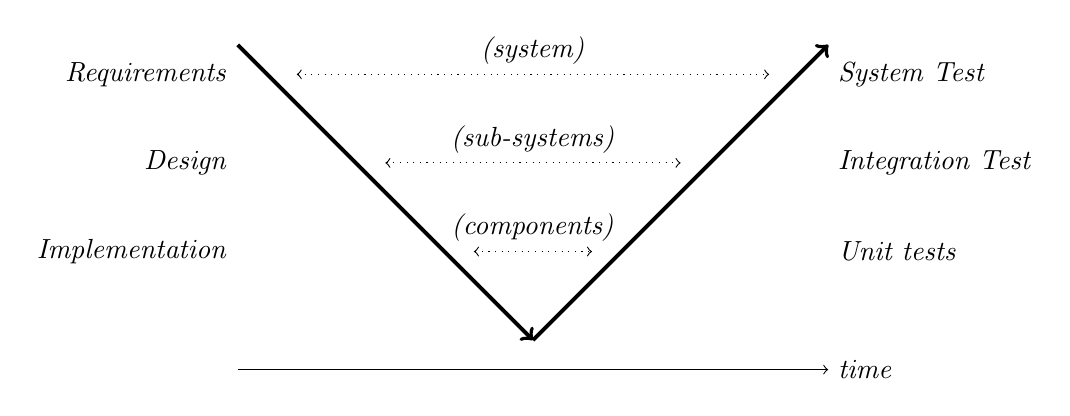
\begin{tikzpicture}[scale=1.5]
        % time arrow
        \draw[->] (0, 0.25) -- (5, 0.25);
        \draw (5, 0.25) node[right] {\textit{time}};
        
        % top to bottom arrow
        \draw[->, line width=0.5mm] (0, 3) -- (2.5, 0.5);
        % bottom to top arrow
        \draw[->, line width=0.5mm] (2.5, 0.5) -- (5, 3);
        
        % system arrow
        \draw[<->, dotted] (0.5, 2.75) -- (4.5, 2.75);
        \draw (2.5, 2.75) node[above] {\textit{(system)}};
        \draw (0, 2.75) node[left] {\textit{Requirements}};
        \draw (5, 2.75) node[right] {\textit{System Test}};
        
        % sub-systems
        \draw[<->, dotted] (1.25, 2) -- (3.75, 2);
        \draw (2.5, 2) node[above] {\textit{(sub-systems)}};
        \draw (0, 2) node[left] {\textit{Design}};
        \draw (5, 2) node[right] {\textit{Integration Test}};
        
        % components
        \draw[<->, dotted] (2, 1.25) -- (3, 1.25);
        \draw (2.5, 1.25) node[above] {\textit{(components)}};
        \draw (0, 1.25) node[left] {\textit{Implementation}};
        \draw (5, 1.25) node[right] {\textit{Unit tests}};
    \end{tikzpicture}
    \caption{Traditional V-Model}
    \label{Traditional V-Model}
\end{figure}

There are three types of tests in the V-Model which correspond to the component, sub-system and system levels.

\subsubsection{Unit tests}

Tests for the components level are called \textit{unit tests}, as they test small self-contained portions of code. This step is required to be able to confirm the validity of the implementation, by testing the code exhaustively\cite{27763}.

The complexity of unit testing comes down to maximizing the exhaustiveness of the tests. Techniques such as \textit{coverage testing} can be used to increase their robustness.

Unit tests are preferred compared to higher level tests for components as it doesn't generally involve too much code and makes the systematic analysis easier\cite{76037}.

\subsubsection{Integration tests}

Once each component has been thoroughly tested separately, \textit{integration tests} make sure that they work well together to be part of a larger sub-system.

Even though these types of test provide a way of testing the interaction between components to diagnose any potential problem, it doesn't help in identifying and understanding the issue\cite{7100358}.

Integration tests also tend to be more difficult to write than Unit tests, that's the reason why there is always less of them.

\subsubsection{System tests}

Making sure that each sub-system can perform together as intended to form the entire \textit{system} can be achieved through \textit{system tests}. They check the behaviour of the system to verify that it meets the previously written specification.

Although these tests are not very common due to their complexity, they can be automated using \textit{Unified Modeling Language} requirement diagrams such as \textit{use case} or \textit{sequence} diagrams\cite{hartmann_uml-based_2005}.

\subsection{Agile software development}
   
    Ever since the Agile Manifesto and its underlying twelve principles were created, the model gained popularity in the industry and among the software engineering community. 

As stated by its authors in the Manifesto of the Agile Alliance, listed below are the Agile values and principles:

 \textbf{\textit{We are uncovering better ways of developing software by doing it, and helping others do it. Through this work we have come to value:}} 
   \begin{itemize}
    \item[-] Individuals and interactions over processes and tools.
    \item[-] Working software over comprehensive documentation
    \item[-] Customer collaboration over contract negotiation
    \item[-] Responding to change over following a plan
   \end{itemize}
    
    Martin Fowler explained "The Essence of Agile Software Development" by saying "Agile Development is adaptive rather than predictive; people-oriented rather than process-oriented.".
    The Agile methodologies transform the software development process. It becomes more adaptable to change and therefore less costly and more time-efficient.
    
    In Agile development, the testing process is directly integrated into the development phase to correct bugs upstream. It helps to identify problems as early as possible and speeds up product deployment\cite{stolberg_enabling_2009}. 
    
    Continuous integration is the practice of continuously integrating changes to a project and testing them at least once a day or more. Typically, each member of a team integrates his or her work at least once a day. Thus, every day, many integrations are made.
    The intended outcome is to identify any problems in the code and automatically notify the developer. This helps ensure that the code base is not broken any longer than necessary\cite{stolberg_enabling_2009}.
    
    Continuous testing is the very important phase of the end-to-end application life cycle management process. It involves functional testing, performance testing, security testing, and so on. Selenium, Appium, Apache JMeter, and many other tools can be utilized for the same.
    
   Above is an example of a possible specification for Agile testing \cite{media_art_nodate}
    \begin{enumerate} 
        \item \textbf{Define and execute “just-enough”
        acceptance tests:} it allows developers to clearly define a functionality and its expected behavior.
    \item \textbf{Automate as close to 100\% of the
acceptance tests as possible:} Running all tests manually can slow down the development process when the application contains thousands of features to be tested. Automating tests saves time and facilitates the integration of new tests.
    \item \textbf{ Automate acceptance tests using a
“subcutaneous” test approach with a xUnit (or an other framework) test framework: } this process makes it possible to ingest the tests in a versioned repository.
    \item \textbf{Run all acceptance tests in the
regression test suite with the build, daily (at
a minimum).} 
    \item \textbf{Develop unit tests for all new code during a
time period.}
    \item \textbf{Run all unit tests with every build.}
    \item \textbf{Run multiple builds per day}
    \end{enumerate}

\newpage

\section{The Box testing approach}
The box testing approach is a way of classifying tests. There are two types of them: \textbf{White box} and \textbf{Black box} testing.
The first one consists of tests which take into consideration the inner workings of a program.
On the other hand, Black box testing is achieved by testing a program from its user's point of view. This candid approach can help identify a broader spectrum of issues.
\subsection{White-box}

\subsubsection{Static and Dynamic code analysis}

Static and Dynamic code analysis are two ways of automatically analysing computer programs. With static program analysis, the code is read but not executed and return information about correctness (partial and total), optimisation and statistics. There are two types of analysis : Data flow analysis which gathers values in the program and Symbolic analysis which us symbolic data tables.
Static analysis can be achieved with linters, it is a static code analysis tool which analyses stylistic and semantic errors in the code. There is a command in Unix, \texttt{lint} (see Unix manual), which allows a user to statically analyze code in C. It detects various errors such as variable which were declared but not used.

Dynamic analysis allows the developer to get information about execution time, memory and power consumption by executing the code. Many tools are available like Address, Leak or Memory sanitizers from the \texttt{llvm} project. It can also detect data races and deadlocks with the ThreadSanitizers.\cite{4815280}

\subsubsection{Code coverage}
In order to know if the amount of tests executed on a program is sufficient and every feature has been verified, we can proceed to do some code coverage measurements. They allow us to calculate the percentage of code executed in our program. It is based on analysing the variables, functions, and function returns to check if they are correct. Developers aim at getting the best code coverage in order to be sure most of the defects have been removed. So it takes time to create unit and integration tests to increase the percentage. However, a 100 percent code coverage does not mean a bug free program. It is important to have decent code coverage to avoid forgetting to test a major functionality. However, relying only on this is insufficient.\cite{8804437}

\subsubsection{Regression testing}
    As software evolves over time, new versions are released regularly. This involves adding new features and making modifications (improving the User interface for example) to satisfy consumers. Regression tests are used to check that the old functionalities are not affected by the new ones, that the modifications have not impacted the well functioning of the software and that there are no new bugs.\cite{regression}
    
    
    

\subsection{Black-box}
%GA une réf serait bien
Black-box testing is a software test method that allows you to detects bugs in a program without knowing the internal structure of the elements tested. There are several types within the Black-box approach, as some bugs cannot be found using just one of them.

\begin{figure}[ht]
    \centering
    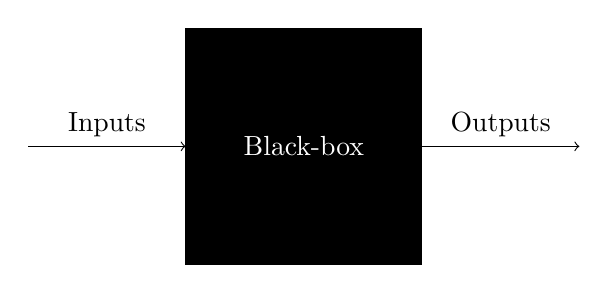
\begin{tikzpicture}[scale=1]
        
        \draw[->] (0, 2) -- (2, 2);
        \draw (1, 2) node[above] {Inputs};
        
        \filldraw[fill=black] (2, 0.5) rectangle (5, 3.5);
        \draw (3.5, 2) node[text=white] {Black-box};
        
        \draw[->] (5, 2) -- (7, 2);
        \draw (6, 2) node[above] {Outputs};
    \end{tikzpicture}
    \caption{Black-box testing}
    \label{fig:black-box testing}
\end{figure}

%GA la figure a la main directement sous Latex, ca c'est impressionnant!

\subsubsection{Fuzz testing}

The term ``fuzz`` was first introduced in the 90s to test the reliability of computer programs. It only received worldwide attention a few years later. Fuzzing or fuzz testing is a software testing technique to reduce defects in software systems or given targets. These numerous faults can generate vulnerabilities exploited by malicious users to attack these systems by executing their own code. "Fuzz testing is a process that sends malformed or semi-valid data to a program deliberately to detect vulnerabilities or errors in the target" \cite{zhang_discover_2018}.

Considering inputs are random, they are likely to reveal inappropriate and unexpected behaviour in the targeted program. The piece of software tested can crash during fuzzing if it does not correctly reject incorrect entries. 

\subsubsection{Decision Table Testing}


The most rigorous functional testing methods are based on decision tables. The decision table test is built on its solid foundation. Since the early 1960s, decision tables have been used to analyze and represent complex logical relationships. "They are ideal for describing situations in which a number of combinations of actions are taken under varying sets of conditions." \cite{jorgensen_decision_2014}

 
A decision table is made up of four distinct parts:
\begin{itemize}
  \item[-] The stub portion
  \item[-] The entry portion
  \item[-] The condition portion
  \item[-] The action portion
\end{itemize}

In decision table \ref{tab:Decision table example}, when conditions \texttt{c1} and \texttt{c2} are True, and condition \texttt{c3} is False, actions \texttt{a1} and \texttt{a3} occur. For Rule 6, \texttt{c1} is wrong, \texttt{c2} is wrong and \texttt{c3}'s value does not have any impact.
A decision table is actually a truth table if the conditions are binary, this guarantees us to take all possible combinations into account.

\begin{table}[ht]
\centering
\begin{tabular}{ |c|c|c|c|c|c|c| } 
\hline
Stub & Rule 1 & Rule 2 & Rule 3 & Rule 4 & Rule 5 & Rule 6 \\
\hline
\hline
\rowcolor{Gray}
c1 & T & T & T & F & F & F \\
\hline
c2 & T & T & F & T & T & F \\
\hline
\rowcolor{Gray}
c3 & T & F & - & T & F & - \\ 
\hline
\hline
a1 & x & x &  & x & &  \\
\hline
\rowcolor{Gray}
a2 & x & & & & x &   \\
\hline
a3 &  & x & & x & &  \\
\hline
\rowcolor{Gray}
a4 &  &  & x & &  & x  \\ 
\hline
\end{tabular}
\caption{Decision table example}
\label{tab:Decision table example}
\end{table}


\subsubsection{State Transition Testing}

State transition testing is a Black-box testing technique. This technique is an improvement of the Decision table, where the output depends on the input conditions and the previous output. This allows developers to analyse more complex behavior such as finite-state machines.

``The two most common coverage criteria used in state transition testing are all states coverage and all transitions coverage. All states coverage criterion requires reaching all states, whereas all transitions coverage criterion requires exercising all transitions.``\cite{de_souza_carvalho_coverage_2014}

\newpage

There are 4 main components of the State Transition Model:
\begin{itemize}
  \item[-] State
  \item[-] Transition
  \item[-] Events
  \item[-] Actions
\end{itemize}

We will take the example of a SIM card. If the PIN code is correct in any of the three attempts, the user will be accepted. If it fails after the third time, the user will be blocked. Also, if the user enters the wrong password the first and two times, we will ask them again.

\begin{figure}[ht]
    \centering
    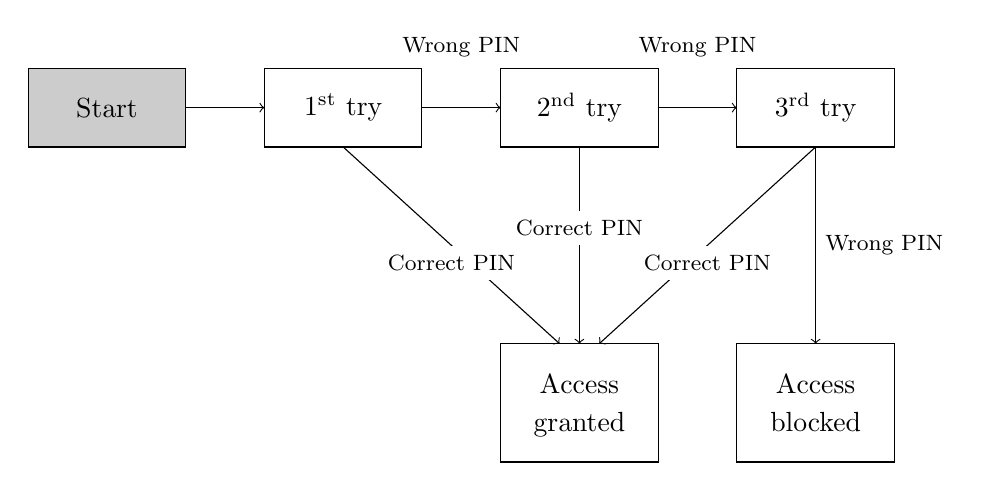
\begin{tikzpicture}[scale=1]
        % start
        \filldraw[fill=black!20] (0, 3) rectangle (2, 4);
        \draw (1, 3.5) node {Start};
        
        \draw [->] (2, 3.5) -- (3, 3.5);
        
        % first try
        \draw (3, 3) rectangle (5, 4);
        \draw (4, 3.5) node {1\textsuperscript{st} try};
        \draw [->] (4, 3) -- (6.75, 0.5) node[midway, below, fill=white] {\footnotesize{Correct PIN}};
        
        \draw [->] (5, 3.5) -- (6, 3.5) node[midway, above=1.5em] {\footnotesize{Wrong PIN}};
        
        % second try
        \draw (6, 3) rectangle (8, 4);
        \draw (7, 3.5) node {2\textsuperscript{nd} try};
        \draw [->] (7, 3) -- (7, 0.5) node[midway, above, fill=white] {\footnotesize{Correct PIN}};
        
        \draw [->] (8, 3.5) -- (9, 3.5) node[midway, above=1.5em] {\footnotesize{Wrong PIN}};
        
        % third try
        \draw (9, 3) rectangle (11, 4);
        \draw (10, 3.5) node {3\textsuperscript{rd} try};
        \draw [->] (10, 3) -- (7.25, 0.5) node[midway, below, fill=white] {\footnotesize{Correct PIN}};
        \draw [->] (10, 3) -- (10, 0.5) node[midway, right] {\footnotesize{Wrong PIN}};
        
        % Access granted
        \draw (6, -1) rectangle (8, 0.5);
        \draw (7, -0.25) node[above] {Access};
        \draw (7, -0.25) node[below] {granted};
        
        % Access blocked
        \draw (9, -1) rectangle (11, 0.5);
        \draw (10, -0.25) node[above] {Access};
        \draw (10, -0.25) node[below] {blocked};
    \end{tikzpicture}
    \caption{State Transition testing \cite{de_souza_carvalho_coverage_2014}}
    \label{fig:state transition testing}
\end{figure}

\newpage

\section{Embedded specific testing}

Simulation techniques are used to test embedded systems. Model-in-the-loop, Software-in-the-loop and Hardware-in-the-loop simulations are the three testing techniques usually set up for verifying the correct functioning of an embedded system.

\subsection{Model In the Loop}


Model-in-the-loop is the first step of the validation process. During this test phase, the entire system is verified using modeling. It allows developers to use virtual simulation on a system via a real-time computer simulation. Thus, thanks to mathematical models, physical testing is not the only solution to testing a mechanical system. To design these models, tools such as MATLAB and Simulink are used.

This technique has many advantages, such as reducing the cost and the complexity of the physical test, and also improving team cohesion and communication, while facilitating the explanations and the agreement with the customer on the various features\cite{MIL_Complex}.
Moreover, component modeling is practical, a system can be tested even if some physical parts are not finished. 

However, to work, the parts simulated with the computer need sensors to communicate with the rest of the system. These will not be present in the real system and can introduce errors. According to A. R. Plummer, "The difficulties associated with limited actuator response have been a major concern"\cite{Model_in_the_loop}, but various solutions have been proposed to counter these delays issues.

\begin{figure}[ht]
    \centering 
   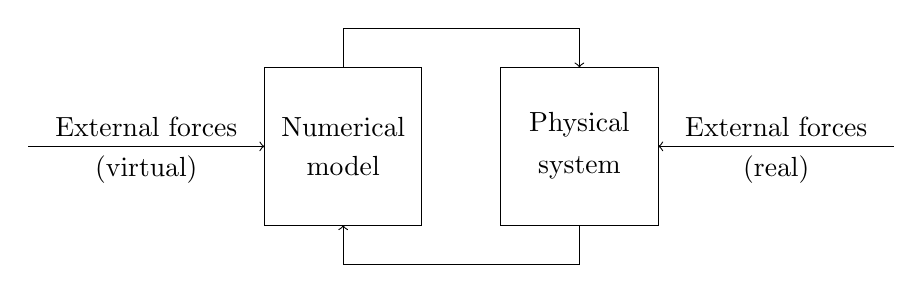
\begin{tikzpicture}[scale=1]
        % ligne
        \draw[->] (-3, 0) -- (0, 0);
        \draw (-1.5, 0) node[above] {External forces};
        \draw (-1.5, 0) node[below] {(virtual)};
        
        \draw (0, -1) rectangle (2, 1);
        \draw (1,0) node[above] {Numerical};
        \draw (1,0) node[below] {model};
        
        \draw (3, -1) rectangle (5, 1);
        \draw (4,0) node[above] {Physical};
        \draw (4,0) node[below] {system};
        
        \draw[<-] (5,0) -- (8,0);
        \draw (6.5, 0) node[above] {External forces};
        \draw (6.5, 0) node[below] {(real)};
        
        \draw[->] (1, 1) -- (1, 1.5) -- (4, 1.5) -- (4, 1);
        \draw[<-] (1, -1) -- (1, -1.5) -- (4, -1.5) -- (4, -1);
      
    \end{tikzpicture}
    \caption{Model-in-the-loop concept\cite{Model_in_the_loop}}
\end{figure}

The MIL method is therefore very useful to simulate a system at the start of a project. During the design phase, engineers can use it to properly define and understand the system. However, it can lack precision and it can not be completely in agreement with the final real system, because it is necessary to use tools to achieve it which can add inaccuracies.




\newpage


\subsection{Software In the Loop}
SIL (Software-In-The-Loop) is a process for performing tests in order to develop and validate an algorithm while being based on a hardware representation of a given system \cite{silva_design_2019}. More precisely, the tests of SIL are employed among manufacturers upstream of the development process \cite{beyer_software_2017}.We can use the V-model to represent where SIL tests are supposed to be done.

\begin{figure}[ht]
    \centering
    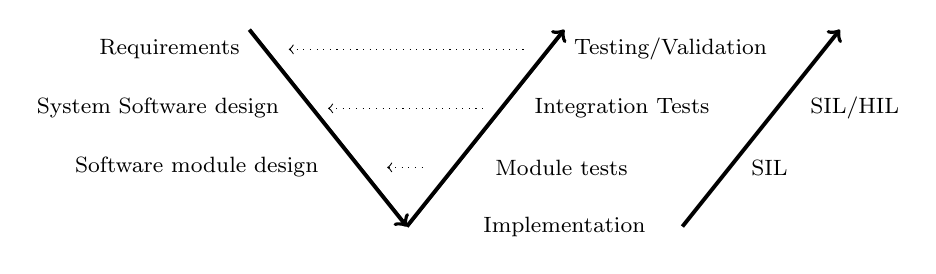
\begin{tikzpicture}[scale=1]
         % top to bottom arrow
        \draw[->, line width=0.5mm] (0, 3) -- (2, 0.5);
        % bottom to top arrow
        \draw[->, line width=0.5mm] (2, 0.5) -- (4, 3);

        
        % system arrow
        \draw[<-, dotted] (0.5, 2.75) -- (3.5, 2.75);
        \draw (0, 2.75) node[left] {\footnotesize{Requirements}};
        \draw (4, 2.75) node[right] {\footnotesize{Testing/Validation}};
        
        % sub-systems
        \draw[<-, dotted] (1, 2) -- (3, 2);
        \draw (0.5, 2) node[left] {\footnotesize{System Software design}};
        \draw (3.5, 2) node[right] {\footnotesize{Integration Tests}};
        
        % components
        \draw[<-, dotted] (1.75, 1.25) -- (2.25, 1.25);
        \draw (1, 1.25) node[left] {\footnotesize{Software module design}};
        \draw (3, 1.25) node[right] {\footnotesize{Module tests}};
        
        % bottom to top arrow
        \draw[->, line width=0.5mm] (5.5, 0.5) -- (7.5, 3);
        
        % components
        \draw (4, 0.5) node {\footnotesize{Implementation}};
        \draw (6.25, 1.25) node[right] {\footnotesize{SIL}};
        \draw (7, 2) node[right] {\footnotesize{SIL/HIL}};
    
        \end{tikzpicture}
    \caption{V-model in an embedded system.}
    \label{V-Model embedded}
\end{figure}



We observe that SIL tests are used in Module tests of Software module design and also in integration tests of System Software design \cite{06384402}.

Software-in-the-loop provides several advantages:  It includes the inexpensive costs and adaptability of a simulator and also the faithfulness of a hardware emulator. Indeed, the cost saving is explained by a high reuse of code and also a low exploitation of development resources \cite{04455268}.

It is the absence of hardware and also that tests are easy to parameter that justify the adaptability of SIL. The fact that we can test the system before the injection in hardware is a good advantage too. This induces a decrease in costs and time dedicated to software testing.

However, the notable drawback is the runtime performance that is not the same as in a real system \cite{beyer_software_2017}.

Despite the fact that software-in-the-loop is an attractive solution for testing, it was not common until recently. Thanks to the appearance of APIs, this testing solution has become widely used \cite{04455268}.






\newpage


\subsection{Hardware In the Loop}


Modern systems grow in complexity, particularly in software where thorough and reliable tests are necessary to verify and validate designs. HIL (Hardware-in-the-loop) is a technique where real signals from a controller are connected to a test system that emulates reality. The solution must provide comprehensive testing as though the real-world system is being used. With the HIL process, you can easily run through thousands of possible scenarios to properly exercise your controller without the cost and time associated with actual physical tests.\cite{065894}

\begin{figure}[h!]
\centering
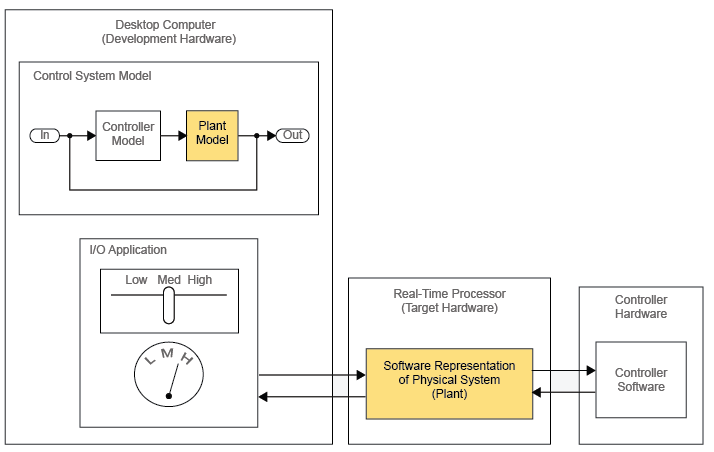
\includegraphics[scale=0.55]{images/HIL.png}
\caption{Hardware-in-the-Loop Simulation setup}
\label{fig:hil}
\end{figure}

The system model is composed of the Development Hardware, the Target Hardware and the Controller Hardware. The Development Hardware contains the model of the physical plant associated with an interface to control the virtual inputs. The Target Hardware contains the code that represents the environment of the tests. The Controller Hardware is associated with SIL.\cite{065893}

The HIL method has its limits. The performance of the test depends on the model implemented. It is complex to implement a precise physical system and a factor of uncertainty is present. To minimize the impact of this factor, it is important to test and validate the design of the controller. The test on the physical plant cannot be seen as the result but as a prediction of what could result. Further tests on the real-model are still important.\cite{On-HIL-simu}

However, HIL simulation offers cost savings over validation testing. It is possible to determine if the plant model is valid and perform design changes earlier in the project which leads to several benefits. You can identify design problems and make changes without the burden of using an assembled final product.\cite{065893}





    

\newpage

\section*{Conclusion}
\addcontentsline{toc}{section}{Conclusion}


In business, two development processes have been widely used: the V-Model and the Agile methods. The choice of process depends on the project. For instance, the Agile methodology allows for more flexibility, in case the client has not clearly defined the product he wants in the first place. This process will ease adding functionalities down the line. The major difference between these two processes lies in the tests. These are directly done alongside the development in the Agile methods, whereas the system is tested once developed for the V-Model. Tests can be classified into two categories according to their characteristics: white-box or black-box.
In the development of embedded systems, simulation techniques such as MIL, SIL and HIL are favored to correct potential errors as they generally reduce costs and cut testing time.

\hspace{1em}

Our mission will be to add functionalities to the Jammer box. We will take care of designing the software, with the development of a driver to manage the storage on an SD card. We will also improve the user interface to be able to easily access and use that data.

We will finally imagine new test scenarios, we could for example test the system against malicious injections.
This is very interesting for modern cars where security is of paramount importance. Indeed, vehicles controlled by software need to be protected against external attacks.
Developers should not only rely on SIL or HIL tests to track down known vulnerabilities. They must anticipate new problems that may arise concerning the safety of the vehicle.


\newpage

\printbibliography